\setboolean{IsHalfPage}{true}%
\setboolean{IsHalfPageLeftCol}{false}%
\setboolean{IsHalfPageRightCol}{true}%
\def\ChapterTitle{%
	Intersecting Dimensions
}
\def\ChapterUrl{%
	https://arnottferels.github.io/work/intersecting-dimensions
}
\def\ChapterDescription{%
	Exploring Anthropocentric \& Analyzing Comfort in a Massive Installation
}
\def\ChapterDetailsLine{%
	Professional Work -- 2021 | Rattan; Shadow Analysis | BSD, Indonesia
}
\def\ChapterDetailsTabular{%
	\begin{tabular}{@{}ll}
		\textbf{Contributions} & Research and Development, Digital Modeling, Analysis and Simulation \& Scripting \\
		\textbf{Software}      & Rhino \& Grasshopper                                                             \\
		\textbf{Team Leader}   & Trianzani Sulshi                                                                 \\
		\textbf{URL}           & \textcolor{blue}{\footnotesize\texttt{\href{\ChapterUrl}{\ChapterUrl}}}          \\
	\end{tabular}
}
\def\ChapterAbstract{%
	This project investigates shadow dynamics in a large installation at Kumulo Creative Compound, BSD. Scheduled for construction from February to April and exhibition until December 2021, it addresses the hot-humid tropical context. The analysis aims to understand shadow interactions, considering limited natural shade, and assesses the design's adaptability to pedestrian traffic and various activities.
}
\def\ChapterFrontmatter{%
	\chapter*{\ChapterTitle}\addcontentsline{toc}{chapter}{\ChapterTitle}
	\ChapterSetTocAddData{\ChapterDetailsLine}
	\ChapterSetDetailsData{\ChapterDescription}{\ChapterDetailsLine}{\ChapterDetailsTabular}
	\RuleAbstract%
	\ChapterAbstract
}
\StartTwoColumnLayout
\raggedright
\begin{minipage}[t][(\PaperHeight-\PaperTopMargin-\PaperBottomMargin
		-16pt%
		)\relax][t]{\linewidth}%
	\ChapterFrontmatter
	\section*{
	  Method
	 }
	%
\begin{figure}[H]
	\centering
	\includesvg[width=\linewidth]{src/graphics/intersecting-dimensions--method-shadow-analysis.svg}
	\label{
		fig:intersecting-dimensions--method-shadow-analysis
	}
\end{figure}

	\vfill
	In BSD, Tangerang, Indonesia, Kumulo is preparing a major installation, with construction scheduled from February to April and the exhibition until December 2021. The study focuses on limited natural shade in the hot-humid tropical area, examining shadows' interaction with the installation and assessing its adaptability. A shadow simulation on June 21, 2021, captures daily patterns, providing insights into impact areas. Preliminary findings guide potential design adjustments for enhanced functionality and aesthetic appeal within Kumulo's hot-humid tropical context.
	\vfill
	\begin{minipage}[t]{0.31\linewidth}%
		%
\begin{figure}[H]
	\centering
	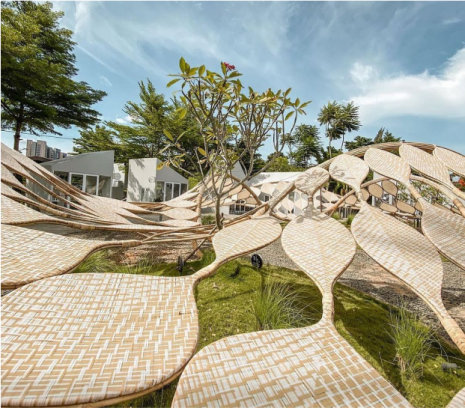
\includegraphics[width=\linewidth]{src/graphics/intersecting-dimensions--fig-03.jpg}
	\label{
		fig:intersecting-dimensions--fig-03
	}
\end{figure}
%
	\end{minipage}
	\hfill
	\begin{minipage}[t]{0.31\linewidth}%
		%
\begin{figure}[H]
	\centering
	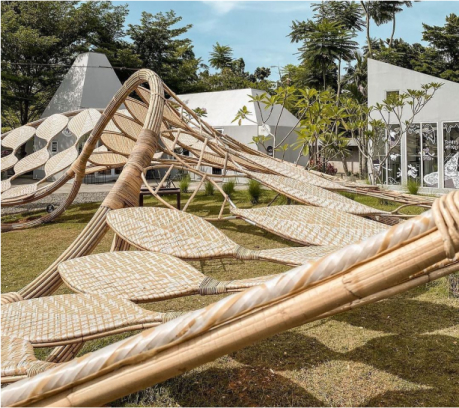
\includegraphics[width=\linewidth]{src/graphics/intersecting-dimensions--fig-02.jpg}
	\label{
		fig:intersecting-dimensions--fig-02
	}
\end{figure}
%
	\end{minipage}
	\hfill
	\begin{minipage}[t]{0.31\linewidth}%
		%
\begin{figure}[H]
	\centering
	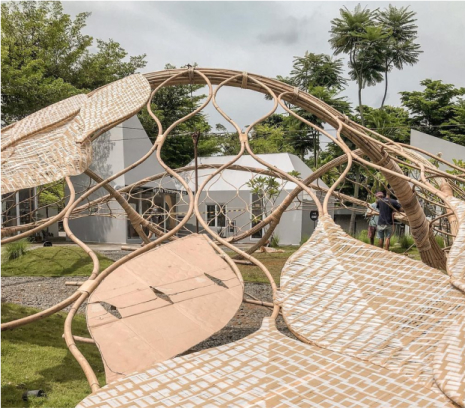
\includegraphics[width=\linewidth]{src/graphics/intersecting-dimensions--fig-01.jpg}
	\label{
		fig:intersecting-dimensions--fig-01
	}
\end{figure}
%
	\end{minipage}
\end{minipage}
\EndTwoColumnLayout
\newpage
